% meta.concepts: beam shear and bending moment diagram
% meta.tags: realistic
% acknowledge: Peter Seiler & Luke Melander graciously shared Spring 2019 course material
% source: 2019 P. Seiler AEM2011 HW 10

The Guthrie Theater, shown below (left), is located on the west bank of the Mississippi River. It
includes a 178 foot bridge. Assume the bridge can be modeled as a cantilevered beam with the
distributed load $w(x)$ as shown below (right). The distributed load is given by
\begin{itemize}
  \item $w(x) = w_0$ lb/ft for $0 \le x \le 150$ ft 
  \item $w(x) = w_0\frac{178-x}{28}$ lb/ft for $150 < x \le 178$ ft
\end{itemize}
Where $w_0$ is a constant with the sign convention $w_0 > 0$ corresponding to the distributed load acting in the $-y$ direction as shown.

Draw the shear and bending moment diagrams for the bridge

\begin{figure*}[ht!]
  \centering
  \includegraphics[width=0.4\textwidth,
	           height=0.3\textheight,
		   keepaspectratio]{figa.png}
  \includegraphics[width=0.4\textwidth,
	           height=0.3\textheight,
		   keepaspectratio]{figb.png}
\end{figure*}

\iftoggle{flagSoln}{%
\vspace{.5cm}
\rule{\textwidth}{.4pt}
\vspace{.5cm}
\textbf{Solution:}
\begin{figure}[ht!]
  \centering
  \frame{\includegraphics[width=0.45\textwidth,
	           height=0.5\textheight,
       keepaspectratio]{solna.png}}
  \frame{\includegraphics[width=0.45\textwidth,
	           height=0.5\textheight,
       keepaspectratio]{solnb.png}}
\end{figure}
}{%
}%
